\section{Marco teórico de referencia y antecedentes}

El marco de referencia está organizado en un primer momento con el análisis del estado del arte para la comprensión del objeto de estudios sobre MLOps para el ámbito agrícola y un segundo momento con los elementos teórico-conceptuales que permiten la argumentación teórica sobre Machine Learning, la metodología MLOps y el cultivo de aguacate Hass con las plagas detalladas para esta investigación.

\subsection{Estado del arte}
Las investigaciones a nivel internacional se describen a continuación:

\begin{longtable}{|p{2cm}|p{3cm}|p{3cm}|p{4cm}|p{3cm}|}

\caption{Investigaciones internacionales}\\
\textbf{Autor} & \textbf{Título} & \textbf{Objetivo} & \textbf{Metodología} & \textbf{Resultado} \\
\hline
\endfirsthead
  \caption[]{Investigaciones internacionales}\\
  \textbf{Autor} & \textbf{Título} & \textbf{Objetivo} & \textbf{Metodología} & \textbf{Resultado} \\
  \hline
\endhead

\citet{aimacana2021} & Análisis comparativo de algoritmos de Machine Learning para la detección de plagas en los cultivos representativos de la sierra ecuatoriana & Realizar un análisis comparativo entre distintos algoritmos de Machine y Deep Learning, que permita determinar cuál de ellos ofrece mejores resultados en la detección de plagas en cultivos endémicos de la serranía ecuatoriana. & Metodología CRISPDM la cual sus siglas significan Proceso Estándar Entre Industrias para la Minería de Datos. & El estudio realizado se aplicó el mejor modelo para la construcción de un prototipo el cual fue la red neuronal convolucional InceptionV3; el prototipo realizado, permite al usuario enviar imágenes para ser procesadas por el modelo y este a su vez reciba una predicción e información de los síntomas, además de una sugerencia de un posible tratamiento. \\
\hline
\citet{castaneda2021} & Detección de nutrientes del suelo y planta, y pestes en campos de cultivo de banano orgánico con Machine Learning & Diseño una plataforma que sirva de apoyo al agricultor para poder estimar qué macronutrientes tiene en deficiencia su planta de banano, con la finalidad de obtener un mejor producto en la cosecha del banano orgánico, así como una posible interfaz para la detección de plagas en el banano. & Se utilizó un conjunto de fotografías público, el cual fue encontrado en un repositorio y se escogieron aquellas plagas que afectaban al banano. Posteriormente, se realizó un aumento a este conjunto de fotografías mediante transformaciones lineales y las imágenes resultantes fueron pre procesadas en diferentes espacios de color para ser utilizadas como entradas a la red neuronal. & El modelo permitió una alta precisión a través de diferentes métricas. Continuamente se desarrolló un prototipo de plataforma web para que los agricultores en un futuro pudieran acceder al sistema. \\
\hline
\citet{valenzuela2022} & Detección y Clasificación de Enfermedades en el Tomate Mediante Deep Learning y Computer Visión & Aplicar el aprendizaje profundo a problemas de visión de computadora tales como detección y clasificación específicamente en las enfermedades del tomate mediante el procesamiento de imágenes digitales. & Redes neuronales pre-entrenadas utilizando transfer learning para llevar a cabo la detección de hojas de tomate, utilizando inicialmente Faster Mask R-CNN, seguido por una red neuronal convolucional para clasificar la enfermedad. Esta clasificación se basa en el área de la imagen donde se ubica la hoja. Una vez clasificada, el sistema proporciona información sobre los síntomas asociados con la enfermedad, así como recomendaciones en tiempo real sobre la prevención y el tratamiento adecuado. & Con el advenimiento de las redes neuronales, ha permitido mejorar drásticamente la precisión, tanto de la detección de objetos como de la clasificación de imágenes. \\
\hline
\citet{garcia2022} & Implementación de modelo Machine Learning aplicado al estudio de enfermedades de café en el centro de investigación Sacha Wiwa, perteneciente a la parroquia Gasaganga, Cantón la Maná, provincia de Cotopaxi & Implementar modelo de clasificación de imágenes empleando técnicas de Machine Learning, para la detección de enfermedades del Cafeto (Coffea arábica) en huertas del Centro de Investigación Sacha Wiwa. & Cualitativa experimental permite la selección, análisis y presentación de los datos documentados de una manera ordenada y siguiendo los objetivos del proyecto. & Utilizando el entorno virtual "Jupyter Lab", se logró desarrollar y entrenar un modelo de Machine Learning que emplea redes neuronales convencionales para clasificar las enfermedades del café mencionadas en el caso de estudio, junto con la clasificación de plantas de café sanas. \\
\hline
\caption*{\footnotesize Fuente: Elaboración propia}
\end{longtable}


En las investigaciones a nivel internacional se puede observar que el desarrollo del Machine Learning, en particular el uso de redes neuronales, ha demostrado ser de gran importancia en el control de plagas y enfermedades en diversos campos, como la agricultura. Asimismo este utiliza un modelo de red neuronal convolucional para la detección de plagas y enfermedades como por ejemplo en los cultivos de café, tomate y banano donde se posibilita que el Machine Learning pueda contribuir al control de plagas.

Uno de los principales beneficios del Machine Learning en el control de plagas es su capacidad para analizar grandes volúmenes de datos y extraer patrones y características relevantes, en las investigaciones se observaron que utilizaban imágenes  de plantas enfermas como sanas, lo que le permitió aprender a reconocer los síntomas y distinguir entre diferentes enfermedades. Esto es especialmente útil en el control de plagas, ya que puede facilitar la detección temprana de enfermedades y ayudar a los agricultores a tomar medidas preventivas o correctivas de manera oportuna.

Para el caso de las investigaciones nacionales se detallan en la siguiente tabla:


\begin{longtable}{|p{2cm}|p{3cm}|p{3cm}|p{4cm}|p{3cm}|}

\caption{Investigaciones a nivel nacional}\\
\textbf{Autor} & \textbf{Título} & \textbf{Objetivo} & \textbf{Metodología} & \textbf{Resultado} \\
\hline
\endfirsthead
	\caption[]{Investigaciones a nivel nacional}\\
	\textbf{Autor} & \textbf{Título} & \textbf{Objetivo} & \textbf{Metodología} & \textbf{Resultado} \\
	\hline
\endhead

\hline
\endfoot

\hline
\endlastfoot

\citet{tovar2019} & Diseño e implementación de un aplicativo móvil para realizar la detección temprana de la enfermedad de la Sigatoka Negra en los cultivos de plátanos & Diseñar e implementar un aplicativo móvil, para realizar la detección temprana de la enfermedad de la Sigatoka Negra en los cultivos de plátanos. & 
La metodología empleada para detectar esta enfermedad implicó la creación de una base de datos que contiene imágenes representativas de sus posibles estados, utilizando la escala estándar de Fouré para analizar la progresión de la Sigatoka Negra. Posteriormente, se desarrolló un algoritmo que segmentó cada una de las imágenes para resaltar la enfermedad, extrayendo luego las características pertinentes. Finalmente, mediante técnicas de aprendizaje automático, se generó un modelo de clasificación capaz de identificar el estado de una hoja al capturar una imagen que no esté en la base de datos. & El aplicativo móvil logró una precisión del 80\% en la identificación de la enfermedad de la Sigatoka Negra. Por ende, esta aplicación tiene el potencial de ser una herramienta valiosa para los productores de plátano al prevenir posibles pérdidas económicas. \\
\citet{avila2022} & Entrenamiento de redes neuronales para la identificación de plagas en cultivos de café. & Implementar un aplicativo basado en visión artificial para la identificación de Cercospora, Phoma, Roya, minador de hojas y Arañita roja, en el café a partir del análisis de las hojas de la planta. & Esta base será introducida a modelos de redes neuronales: densa, neuronal convolucional y neuronal convolucional con overfitting, usando el lenguaje Python y las bibliotecas: Keras y TensorFlow. Una vez entrenado el modelo, se procede al análisis de las imágenes que contienen la morfología de la planta y que servirán de entrada a una red neuronal para poder comparar los resultados y determinar cuál de los modelos presenta mejores resultados. & El modelo convolucional con overfitting ofrece la mejor capacidad predictiva, aunque sigue siendo un modelo restringido que podría ser sustituido por otros modelos más amplios, como ResNet50, CIFAR-10 o VGG19. Dado el número limitado de plagas disponibles, es claro que el reconocimiento detallado de las plagas no es factible en la actualidad, lo que resalta la necesidad de expandir la base de datos. \\
\hline
\caption*{\footnotesize Fuente: Elaboración propia}
\end{longtable}

A nivel nacional los diferentes modelos operativos en el contexto de la detección de plaga hace referencia a un modelo convolucional con overfitting que presenta los mejores resultados de predicción, pero se plantea la posibilidad de reemplazarlo por otros modelos de mayor alcance, como ResNet50, CIFAR-10 o VGG19.

La elección del modelo operativo es crucial en cualquier aplicación de Machine Learning, ya que tiene un impacto directo en la precisión y el rendimiento del sistema. En el caso mencionado, el modelo convolucional con overfitting logró un alto nivel de acierto en la detección de plaga.

\subsection{Bases teóricas}
\subsubsection{Metodología MLOps}

Machine Learning Operations (en sus siglas en inglés MLOps) es un conjunto de prácticas que combinan Machine Learning, DevOps e Ingeniería de datos, cuyo objetivo es implementar y mantener sistemas ML en producción de manera confiable y eficiente.
 
En esa dirección Rivero (\citeyear{rivero2022}) explica que, MLOps se refiere a las prácticas y metodologías que permiten gestionar y optimizar el ciclo de vida de los sistemas de aprendizaje automático (Machine Learning) de forma que se puede desarrollar confiablemente. Se tiene en cuenta que, la metodología MLOps combina técnicas y herramientas de desarrollo de software con conocimientos de ciencia de datos y operaciones de infraestructura, para permitir la implementación, el monitoreo y el mantenimiento escalable de los modelos de aprendizaje automático en producción.

En el contexto del desarrollo de modelos de Machine Learning, MLOps aborda los desafíos asociados con la gestión de datos, la experimentación, el entrenamiento, la implementación, el monitoreo y la reevaluación continua del rendimiento del modelo, que lo hacen diferente a DevOps y la Ingenieria de Datos como se describe en la Tabla \ref{tab:practicas}. Esto implica el uso de técnicas como la integración y entrega continua (CI/CD), la orquestación de flujos de trabajo, la automatización de pruebas y la gestión de versiones.

\begin{table}[h]
\centering
\caption{Comparativo entre DevOps, Ingeniería de Datos y MLOps}
\label{tab:practicas}
\begin{tabular}{|p{3cm}|p{3cm}|p{3cm}|p{4cm}|}
\hline
\textbf{Práctica} & \textbf{DevOps} & \textbf{Ingeniería de Datos} & \textbf{MLOps} \\
\hline
Control de versiones & Versionamiento de código & Versionamiento de código linaje de datos & Versionamiento de código + datos + modelos (conectados) \\
\hline
Pipeline & n/a & Flujo de datos/ETL & Flujo de ML de entrenamiento, flujo de ML para predicción \\
\hline
Validación de comportamiento & Pruebas unitarias & Pruebas unitarias & Validación de modelo \\
\hline
CI/CD & Despliegue de código en producción & Despliega código en flujo de datos & Despliegue de código a producción + Flujo de datos de ML \\
\hline
Validación de datos & n/a & Validación de negocio y formato & Validación estadística \\
\hline
Monitoreo & Basados en SLOs & Basados en SLOs & SLOs + monitoreo diferencial y estadístico \\
\hline
\end{tabular}
\caption*{\footnotesize Fuente: \citet{rivero2022}}
\end{table}

\newpage

El objetivo fundamental de MLOps es garantizar que los modelos de aprendizaje automático sean confiables, reproducibles y escalables en entornos de producción. Al adoptar prácticas de MLOps, las organizaciones pueden acelerar el tiempo de comercialización de sus modelos, mejorar la colaboración entre equipos multidisciplinarios, minimizar los riesgos asociados con los modelos en producción y facilitar la implementación de mejoras y actualizaciones. Estos avances en la metodología MLOps se vienen desarrollando desde el año 2000 para resolver los distintos problemas para los contextos ML (ver figura \ref{fig:figura2}).\\


\begin{figure}[h]
\caption{Evolución temporal de MLOps}
\centering
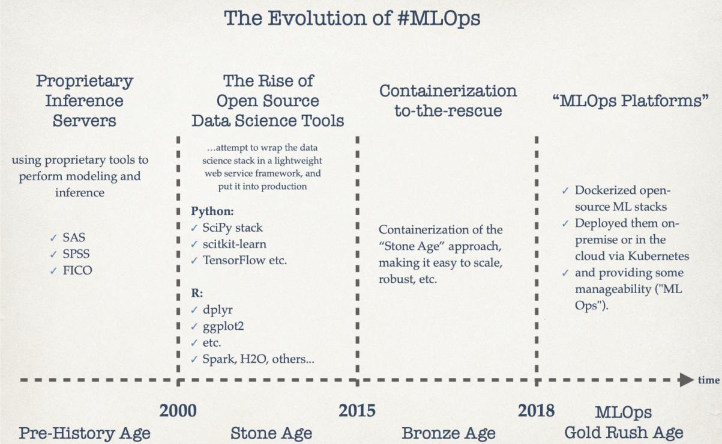
\includegraphics[width=1\textwidth]{evolucionTemporalMLOPS.png}
\label{fig:figura2}
\caption*{\footnotesize Fuente: \citet{visengeriyeva2020}}
\end{figure}


\newpage
La metodología MLOps es una disciplina que fusiona las mejores prácticas de desarrollo de software con los desafíos específicos del Machine Learning, con el objetivo de facilitar la implementación y gestión de modelos de aprendizaje automático. 

Con la creciente popularidad del software de código abierto y la amplia disponibilidad de datos, un número cada vez mayor de profesionales en el campo del desarrollo de software optaron por utilizar bibliotecas en lenguajes como Python o R para llevar a cabo el entrenamiento de modelos de aprendizaje automático. A medida que avanzaba la tecnología de la contenerización, surgió una solución para abordar el despliegue escalable de modelos mediante el uso de contenedores Docker y Kubernetes. En tiempos recientes, hemos observado una evolución en estas soluciones, que ahora han dado paso a plataformas de implementación de aprendizaje automático que abarcan todo el ciclo de vida del modelo, desde la experimentación inicial, pasando por el entrenamiento, la implementación y hasta el monitoreo continuo del rendimiento del modelo \citep{visengeriyeva2020}.
\newpage

\subsubsection{Proceso de la metodología MLOps}
\begin{itemize}
\item \textbf{Flujos de ML:} Los procesos de flujo de datos, conocidos también como pipelines de datos o ETL (extraer, transformar y cargar), implican la obtención de datos desde una fuente, su posterior transformación y finalmente su carga en la misma fuente original o en otro sistema. La fase de transformación de los datos abarca todas las modificaciones necesarias para garantizar que los datos estén en el formato requerido por el destino final, que en este caso sería el modelo de aprendizaje automático.
\item \textbf{Versionado de modelos y de datos:} En aprendizaje automático es crucial, ya que no solo implica mantener un registro de las distintas versiones del código, sino también de las versiones del modelo en sí mismo, así como de los conjuntos de datos utilizados en su entrenamiento, junto con otros detalles como los hiper-parámetros del modelo.
\item \textbf{Validación de modelos:} Se debe tener en cuenta:
    \begin{enumerate}
        \item \textbf{Precisión del modelo:} de los casos que el modelo clasificó como verdaderos positivos (TP).
        \item \textbf{Recall del modelo:} la precisión abierta por categorías.
        \item \textbf{Medición de sesgo en los datos:} es importante realizar mediciones que ayuden a entender si el modelo está sesgado.
        \item \textbf{Casos críticos:} un modelo puede tener buena precisión, exhaustividad(recall) y no estar sesgado, pero no tomar los casos más importantes en la historia reciente.
        \item \textbf{Medición de un modelo de regresión:}\\

- Evaluación general del modelo mediante métricas como RMSE, MAE y R2.\\
- Desglose de estas métricas por diferentes segmentos para identificar áreas donde el modelo podría necesitar mejoras específicas.\\
- Análisis del sesgo presente en los datos, similar al enfoque utilizado en problemas de clasificación.\\
- Identificación casos críticos, empleando un enfoque similar al utilizado en problemas de clasificación.\\
    \end{enumerate}
\item \textbf{Validación de datos:} Se realiza en dos etapas. La primera etapa, más elemental, implica evaluar la calidad de los datos, lo que incluye verificar la cantidad de valores nulos, el cumplimiento del acuerdo de nivel de servicio (SLA) para la actualización de los datos, asegurando que todos los datos sean del tipo esperado, entre otros aspectos. La segunda etapa, más compleja, implica monitorear la distribución de los datos. Cualquier cambio en esta distribución podría deberse a un fallo en alguno de los pipelines o a cambios en los datos mismos. \citep{rivero2022}. 
\end{itemize}

Entre las diversas herramientas disponibles para el MLOps, se pueden clasificar en dos categorías distintas: las sencillas y las complejas. Las herramientas sencillas son particularmente útiles para facilitar el despliegue local, es decir, en un mismo ordenador o un servidor local. Este enfoque es especialmente adecuado para equipos pequeños de investigación, donde estos miembros del equipo pueden acceder desde diferentes computadoras de manera local. Estas herramientas sencillas representan el primer paso para llevar la solución a la fase de despliegue, especialmente en entornos de producción.

Por otro lado, las herramientas complejas están diseñadas para gestionar mayores capacidades de cómputo. Estas pueden configurarse con capacidades específicas, e incluso el sistema puede autoajustarse según el tráfico y los requisitos de almacenamiento, incorporando la funcionalidad conocida como ``On Demand'', donde son capaces de autoescalar según las necesidades del momento. 

Después de implementar las herramientas sencillas, se puede aprovechar lo creado para desplegar una aplicación. Esta aplicación, inicialmente desarrollada o creada localmente, puede integrarse con uno de los servicios en la nube más comunes y populares. Estos servicios en la nube, como AWS, Azure, GCP, son seleccionados debido a su amplia cuota de mercado y su uso generalizado en la actualidad. Esto permite llevar la aplicación creada localmente a aprovechar las capacidades y escalabilidad que ofrecen los servicios en la nube para su despliegue.

\newpage

La implementación de un monitoreo completo plantea ciertas consideraciones, especialmente cuando se considera la adopción de herramientas complejas. La complejidad de estas herramientas conlleva un aumento en los costos, ya que se aplican cargos por el conjunto completo de funcionalidades que ofrecen. En comparación, al optar por el uso de herramientas sencillas locales y utilizar solo una fracción de las herramientas complejas resulta más económico.

Además del aspecto financiero, es crucial tener en cuenta que el uso de herramientas complejas implica una curva de aprendizaje significativa. Se requiere una inversión de tiempo y esfuerzo para adquirir los conocimientos necesarios y comprender cómo manipular eficazmente todo el ciclo del MLOps. Esta curva de aprendizaje elevada puede representar una desventaja, ya que impone una barrera para aquellos que buscan implementar estas herramientas de manera efectiva.

En general, se han ido desarrollando muchas herramientas que se pueden utilizar para implementar la metodología de MLOps tanto de acceso libre (open source) o de pago, para usar localmente o desde internet. Y se deben escoger cada una con base a las necesidades del proyecto.

\begin{figure}[h]
	\centering
	\caption{Herramientas que implementan ciclo completo de MLOps}
	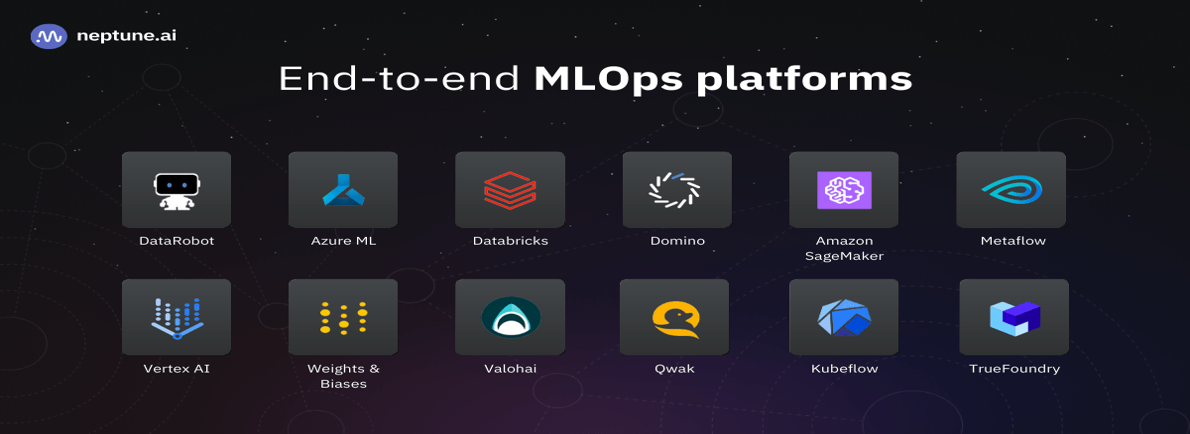
\includegraphics[width=0.8\textwidth]{resultados/herramientasMLOps.png}
	\caption*{\footnotesize Fuente: \cite{neptune2024}}
	\label{fig:figuraHerramientasMLOps}
\end{figure}

\newpage

Dentro de las plataformas descritas en la imagen anterior (ver figura \ref{fig:figuraHerramientasMLOps}) se encuentra MetaFlow, esta plataforma en sí misma, es una herramienta gratuita, aunque algunas de sus funcionalidades pueden requerir pagos. Por ejemplo, el despliegue en internet podría estar sujeto a tarifas adicionales. Para completar todo el ciclo de vida del MLOps, es necesario considerar diversas herramientas, muchas de las cuales ofrecen características completas o parciales para gestionar eficazmente este ciclo.

\begin{figure}[h]
	\centering
	\caption{Herramientas de análisis de datos y repositorio de código}
	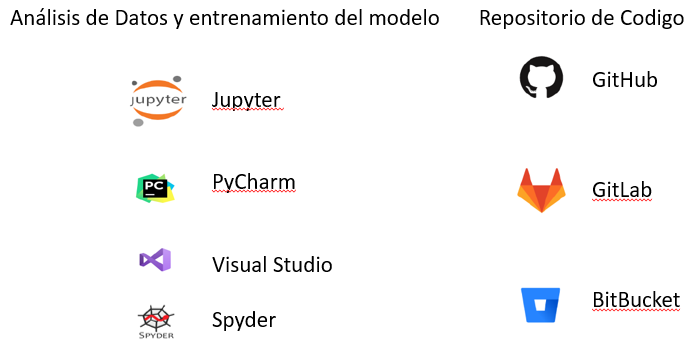
\includegraphics[width=0.7\textwidth]{resultados/herramientasAnaRepo.png}
	\caption*{\footnotesize Fuente: Elaboración propia}
	\label{fig:figuraHerramientasAnaRepo}
\end{figure}

\newpage

\begin{figure}[h]
	\centering
	\caption{Herramientas de registro de modelo, versionado del modelo y versionado de datos}
	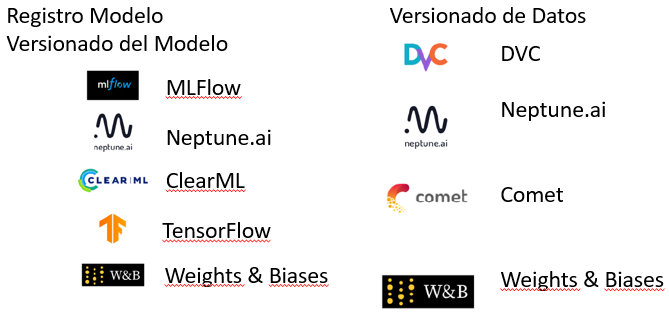
\includegraphics[width=0.7\textwidth]{resultados/herramientasRegModDatos.png}
	\caption*{\footnotesize Fuente: Elaboración propia}
	\label{fig:figuraHerramientasRegModDatos}
\end{figure}

\begin{figure}[h]
	\centering
	\caption{Herramientas para Construcción de API y Construcción de aplicación Web}
	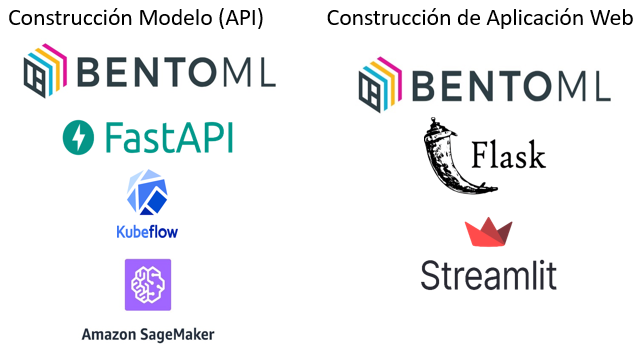
\includegraphics[width=0.6\textwidth]{resultados/herramientasDespApiApp.png}
	\caption*{\footnotesize Fuente: Elaboración propia}
	\label{fig:figuraHerramientasDespApiApp}
\end{figure}

\newpage

\begin{figure}[h]
	\centering
	\caption{Herramientas de Feature Store y Monitoreo del Modelo}
	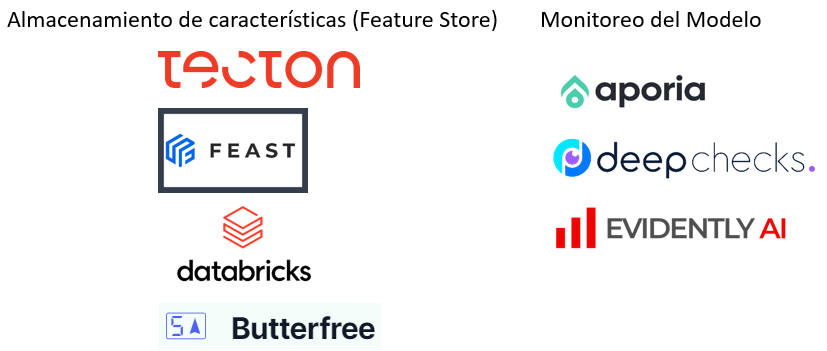
\includegraphics[width=0.9\textwidth]{resultados/herramientasFeaMon.png}
	\caption*{\footnotesize Fuente: Elaboración propia}
	\label{fig:figuraHerramientasFeaMon}
\end{figure}

Continuando con el tema, centrémonos ahora en las herramientas que simplifican los despliegues de una aplicación o una API de manera automatizada. La necesidad de estas herramientas radica en lo tedioso que implicaría realizar despliegues manualmente. En un enfoque manual, se tendría que especificar la imagen que debe utilizarse desde un contenedor, crear el contenedor, y posteriormente enviarlo a la nube. Luego, sería necesario obtener la URL para su uso. Este proceso, aunque es posible de realizar manualmente, se vuelve más eficiente y menos propenso a errores al utilizar herramientas como GitHub Actions, la cual es una herramienta de automatización integrada con GitHub.

Algunas características clave y conceptos asociados con GitHub son:

\begin{itemize}
	\item \textbf{Repositorios:} Son espacios donde se almacenan los archivos de un proyecto,  junto  con  la  información  de  seguimiento  de  versiones.  Cada  proyecto  en GitHub se guarda en un repositorio.
	\item \textbf{Control de Versiones:} GitHub utiliza Git, un sistema de control de versiones distribuido. Esto significa que cada desarrollador o miembro de un equipo, que trabaja en un proyecto tiene una copia completa del historial de cambios del proyecto en su  máquina  local.  Git  permite  rastrear  cambios,  fusionar  contribuciones  y  revertir  a versiones anteriores del código.
	\item \textbf{Automatización:} GitHub Actions es un servicio que permite a los ingenieros de software automatizar diversas tareas en respuesta a eventos específicos dentro del repositorio. En el contexto del proyecto, las tareas se configuran mediante flujos de trabajo definidos en archivos YAML. Estos flujos de trabajo simplifican la ejecución de pruebas, la construcción de una API o una aplicación, junto con los despliegues. GitHub Actions no solo facilita la automatización de estos procesos, sino que también respalda la integración continua y el despliegue continuo.
	
	Esta integración automatizada con GitHub Actions no solo agiliza el ciclo de desarrollo, sino que también asegura la coherencia y confiabilidad en el proceso de despliegue de una aplicación o una API. Con esta herramienta, se logra una gestión eficiente y automatizada de todo el ciclo de vida del modelo para llevarlo a producción, desde la integración de cambios hasta la entrega y despliegue en un proveedor de servicios en la nube.
\end{itemize}

\subsection{Modelo de Machine Learning}

De acuerdo con \cite{salamanca2021}, el modelo Machine Learning se refiere a la localización automatizada de datos que se encuentran estandarizados, además es una herramienta constante en el proceso de extracción de grandes volúmenes de información para su organización y análisis, definido también como Big Data. En la actualidad el Machine Learning es un campo extenso que abarca diversas estrategias analíticas. Su objetivo principal es desarrollar algoritmos capaces de extraer información valiosa de los datos, ya sea para explicar, clasificar o predecir fenómenos \citep{pedro2021}.

Estas nuevas tecnologías, a través del internet, permiten la recopilación de bases de datos de un tamaño considerable, pueden ser históricos o datos en tiempo real, siendo posible el análisis de datos debido a las mejoras constantes en la tecnología y el desarrollo de software. Para \cite{salamanca2021}, este desarrollo ha permitido que las bases de datos se encuentren en distintos formatos, lo que es un desafío para orientar estrategias que permitan resolver distintos problemas de acuerdo a las necesidades de cada formato y de esta manera avanzar en el desarrollo de métodos para el Machine Learning.

Por esta razón con el Machine Learning es posible establecer tres tipos de modelos el geométrico, el probabilístico y el lógico (ver tabla \ref{tab:modelos}) y tres tipos de aprendizajes: el supervisado, el no supervisado y semi-supervisado (ver tabla \ref{tab:tipos}), ya que se busca el aprendizaje continuo, conocer el progreso y la veracidad de la información que se desarrolla, porque:

\begin{quote}
   Su aplicación está determinada en diferentes ámbitos dependiendo de las necesidades del problema, permitiendo a los científicos y especialistas tomar decisiones referentes a temas tan puntales como si un tipo de material puede ser separado por características de resistencia a la fragmentación o capacidad de absorción de energía pudiendo determinar con esto si es recomendable su uso en una u otra tarea específica \citep[p.42]{salamanca2021}.
\end{quote}

\begin{table}[htbp]
\centering
\caption{Modelos para el desarrollo de Machine Learning}
\label{tab:modelos}
\begin{tabular}{|l|p{10cm}|}
\hline
\textbf{Modelo} & \textbf{Características} \\
\hline
Geométrico & El espacio de instancias abarca la totalidad de las configuraciones concebibles, ya sea que estén representadas en nuestro conjunto de datos o no. Suele exhibir una estructura geométrica definida. Por ejemplo, cuando todas las características son de naturaleza numérica, cada una puede interpretarse como una coordenada en un sistema cartesiano. \\
\hline
Probabilístico & Numerosos modelos se sustentan en el siguiente concepto fundamental: Consideremos X como las variables que describen, por ejemplo, las características de una instancia conocida; mientras que Y representa las variables objetivo que nos conciernen, como la clase a la que pertenece dicha instancia. La esencia del aprendizaje automático radica en la capacidad de modelar la interrelación entre X e Y. \\
\hline
Lógico & Toma su inspiración de disciplinas como la informática y la ingeniería. Se denomina ``lógico" debido a que sus modelos pueden ser traducidos de manera sencilla en reglas comprensibles para los seres humanos, por ejemplo: \begin{verbatim}
if Viagra=1 then Class=Y=spam
\end{verbatim} \\
\hline
\end{tabular}
\caption*{\footnotesize Fuente: \citet[p.43]{salamanca2021}}
\end{table}

\begin{table}[htbp]
\centering
\caption{Los tipos de aprendizaje en el ML}
\label{tab:tipos}
\begin{tabular}{|p{4cm}|p{10cm}|}
\hline
\textbf{Tipos} & \textbf{Fundamento} \\
\hline
Aprendizaje supervisado & Consta de descubrir el clasificador óptimo $f: X \rightarrow Y$ para una problemática específica. El proceso para encontrar este mapeo se conoce como algoritmo de clasificación, el cual genera un modelo para cada instancia de entrada $x \in X$ y su correspondiente clase $y \in Y$. Este modelo representa una aproximación de la distribución de probabilidad conjunta (DPC) de las variables $X$ e $Y$. \\
\hline
Aprendizaje no supervisado & Se refieren a casos en los que el objetivo no es ajustar relaciones entre pares de datos de entrada y salida, sino en aumentar el entendimiento estructural de los datos disponibles (y de posibles datos futuros derivados del mismo fenómeno). Por ejemplo, esto podría implicar agrupar los datos en función de su similitud (clustering), simplificar sus estructuras manteniendo sus características esenciales (como en procesos de reducción de dimensionalidad), o extrayendo la estructura interna mediante la cual los datos se distribuyen en su espacio original (aprendizaje topológico). \\
\hline
Aprendizaje semi supervisado & El objetivo es la clasificación, pero la entrada contiene datos etiquetados y sin etiquetar. El aprendizaje semi-supervisado, debido a su estructura, se puede dividir principalmente en dos tipos, según el objetivo del análisis que se busque hacer a la base de datos:
\begin{minipage}[t]{\linewidth}
    \begin{enumerate}
      \item Aprendizaje transductivo, que separa el conjunto dado en conjunto de entrenamiento (donde la variable objetivo es conocida), y conjunto de prueba donde ésta no es dada.
      \item Aprendizaje inductivo trata de obtener una función de predicción usando todo el conjunto $\{(X, Y)\}$, es decir, usando tanto los datos donde la variable objetivo es conocida como aquellos en los que no.
    \end{enumerate}
\end{minipage} \\
\hline
\end{tabular}
\caption*{\footnotesize Fuente: \citet[p.44-45]{salamanca2021}}
\end{table}

\newpage
Autores como \citet{contreras2022}, \citet{salamanca2021} y \citet{jara2016} explican que, en el campo del Machine Learning los métodos de predicción presentan un papel fundamental al permitir que las máquinas realicen predicciones precisas sobre datos no vistos. Existen varios métodos utilizados en el Machine Learning para generar predicciones, entre ellos se destacan los siguientes:

\begin{enumerate}
    \item Regresión: Es utilizado para predecir un valor numérico continuo basado en variables independientes. Algunos ejemplos comunes son la regresión lineal y la regresión logística, que se utilizan para predecir la relación entre variables \citep{salamanca2021}.
    \item Clasificación: Se utiliza para predecir la pertenencia a una clase o categoría específica. Los algoritmos de clasificación, como el árbol de decisiones, las máquinas de vectores de soporte (SVM) y los clasificadores de Naive Bayes, se emplean para clasificar datos en categorías predeterminadas \citep{salamanca2021}.
    \item Agrupamiento: Es utilizado para agrupar conjuntos de datos similares en clusters o grupos. Algunos métodos comunes de agrupamiento son el algoritmo k-means y el agrupamiento jerárquico, que ayudan a encontrar patrones y estructuras ocultas en los datos \citep{contreras2022}.
    \item Redes neuronales: Estas técnicas se basan en modelos inspirados en el funcionamiento del cerebro humano. Las redes neuronales profundas, como las redes neuronales convolucionales (CNN) y las redes neuronales recurrentes (RNN), han logrado grandes avances en áreas como la visión por computadora y el procesamiento del lenguaje natural \citep{salamanca2021}.
\end{enumerate}

Estos métodos de predicción en el Machine Learning han demostrado ser eficientes en una amplia gama de aplicaciones, desde la detección de fraudes hasta el diagnóstico médico y la recomendación de productos. La elección del método adecuado depende del tipo de datos, el problema a resolver y los objetivos específicos del proyecto de Machine Learning. Para verificar su eficiencia, estos métodos deben ser validados por una matriz de confusión la cual contiene:

\begin{figure}[h]
	\centering
	\caption{Matriz de confusión para la evaluación de los modelos}
	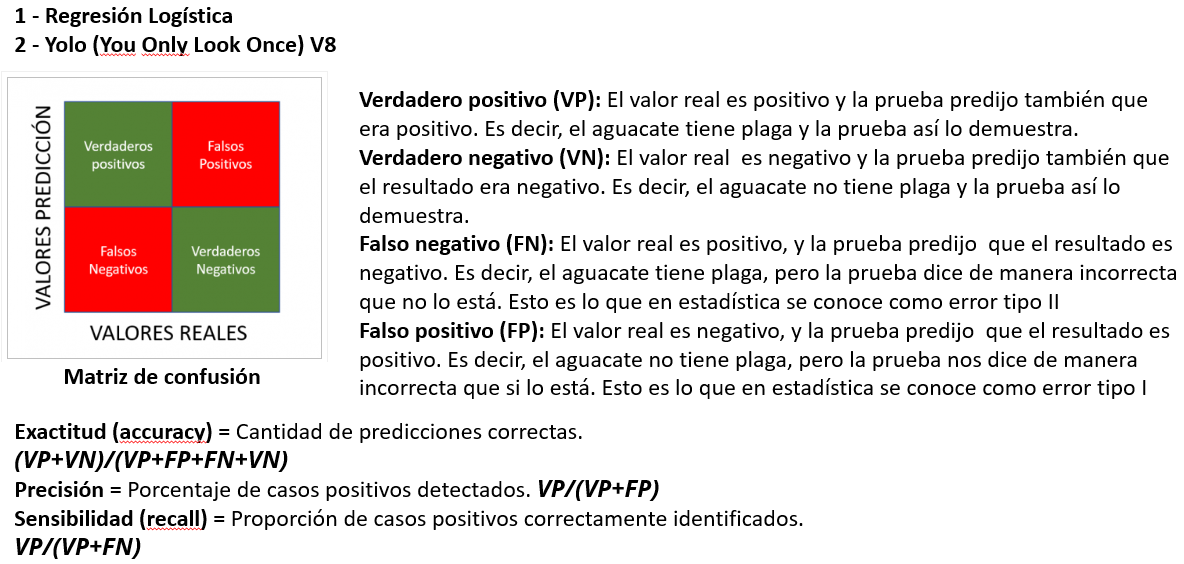
\includegraphics[width=1\textwidth]{resultados/evaModelos.png}
	\caption*{\footnotesize Fuente: Elaboración propia}
	\label{fig:figuraEvaModelos}
\end{figure}

\newpage


\subsubsection{Cultivo de aguacate Hass}

El cultivo del aguacate HASS es cada vez más popular en la agricultura debido a sus características y beneficios. El aguacate HASS es una variedad de aguacate que se distingue por su adaptabilidad a diferentes condiciones climáticas y su alta productividad. Según estudios realizados por el Departamento Administrativo de Nacional de Estadística \citep{dane2016cultivo}, esta variedad se ha destacado por su resistencia a enfermedades y plagas comunes en el cultivo del aguacate.

Una de las ventajas de cultivar el aguacate Hass es su capacidad para adaptarse a diferentes climas, según los autores \citet{reyes2022}, esta variedad es apta para regiones con temperaturas que oscilan entre los 10 y 35 grados Celsius. Además, puede tolerar tanto condiciones secas como húmedas, lo que la convierte en una opción viable para diferentes áreas geográficas.

Cabe destacar, que  otra de las características  del aguacate Hass es su alta productividad, esta variedad puede alcanzar rendimientos superiores a los 20 kilogramos de fruta por árbol al año, esto la convierte en una opción rentable para los agricultores, ya que pueden obtener una mayor producción por unidad de superficie cultivada \citep{reyes2022}.

Además de su adaptabilidad y productividad, el aguacate Hass presenta resistencia a enfermedades comunes en el cultivo del aguacate, según los autores \citet{agapito2022}, esta variedad ha mostrado resistencia al hongo Phytophthora cinnamomi, causante de la pudrición de raíz, lo que reduce la necesidad de aplicar productos químicos para su control.

\subsubsection{Plagas \textit{Stenoma catenifer} y \textit{heilipus lauri}}

El cultivo del aguacate puede verse amenazado por diversas plagas que pueden afectar tanto las hojas, los frutos como las raíces de la planta, según  el Dane  (\citeyear{dane2016cultivo}) las plagas más comunes son el ácaro del aguacate entre los que se encuentran el \textit{Heilipus lauri} y el \textit{Stenoma catenifer}, quienes provoca un daño en la apariencia de la planta y puede reducir su capacidad de fotosíntesis, para controlar esta plaga, se pueden emplear insecticidas específicos o realizar una poda adecuada de las hojas afectadas.

Para \citet{carabali2022}, en el cultivo del aguacate Hass la \textit{Stenoma catenifer} (ver figura \ref{fig:figuraStenoma}) desarrolla su polilla al alimentarse de los frutos del aguacate, perforando galerías y causando daños considerables en la calidad de la cosecha. Asimismo la plaga del barrenador del hueso del aguacate \textit{Heilipus} spp (ver figura \ref{fig:figuraHeilipus}), puede causar daños graves al cultivo, las  larvas de este insecto se alimentan del interior del hueso del aguacate, lo que afecta el desarrollo adecuado del fruto \citep{carabali2022}.

\newpage

\begin{figure}[h]
\centering
\caption{Fotografía del insecto \textit{Stenoma catenifer}}
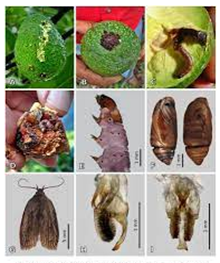
\includegraphics[width=0.33\textwidth]{stenoma.png}
\caption*{\footnotesize Fuente: \cite{diaz2017}}
\label{fig:figuraStenoma}
\end{figure}

\begin{figure}[h]
\centering
\caption{Fotografía del insecto \textit{Heilipus lauri}}
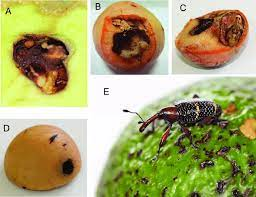
\includegraphics[width=0.42\textwidth]{heilipusLauri.png}
\caption*{\footnotesize Fuente: \cite{palacios2011}}
\label{fig:figuraHeilipus}
\end{figure}